\section{Multi-Stage Training Pipeline Composition}
\label{app:pipeline}

This appendix analyzes multi-stage training pipelines where a large teacher model is first trained on oracle-preserving summaries, then distilled to a smaller student model. We show that training gaps compose additively, providing end-to-end guarantees.

\subsection{Implementation Map}
\begin{itemize}[nosep]
    \item \textbf{Pipeline orchestrator}: \texttt{src/training/run\_pipeline.py} (phases, checkpoints, output layout).
    \item \textbf{Document processing}: \texttt{src/pipelines/batched.py}, \texttt{src/core/batch\_processor.py}, \texttt{src/core/batch\_orchestrator.py}, \texttt{src/tree/builder.py}.
    \item \textbf{Preference collection}: \texttt{src/training/preference/collector.py} and \texttt{src/training/preference/types.py}.
    \item \textbf{Judges and GenRM}: \texttt{src/training/judges/*}, \texttt{src/training/preference/genrm.py}.
    \item \textbf{Optimization}: \texttt{src/training/optimization/*} with configuration in \texttt{src/training/config.py}.
    \item \textbf{Unified/iterative loops}: \texttt{src/training/unified\_trainer.py}, \texttt{src/training/audit\_driven\_training.py}.
    \item \textbf{Dynamic GPU orchestration (optional)}: \texttt{src/core/gpu\_orchestrator.py}.
\end{itemize}

\subsection{CLI and Configuration Mapping}

\paragraph{Shell script entry point.}
\texttt{scripts/run\_training\_pipeline.sh} is the default runner; it builds an
output directory under \texttt{data/results/<task>/training\_pipeline/run\_*}
and calls \texttt{python -m src.training.run\_pipeline} with matching flags.
The Python entry point requires \texttt{--output-dir}; the shell script computes
and supplies this path automatically.

\begin{center}
\begin{tabular}{lll}
\toprule
\textbf{Shell Flag} & \textbf{run\_pipeline Arg} & \textbf{Effect} \\
\midrule
\texttt{--task}, \texttt{--dataset} & \texttt{--task}, \texttt{--dataset} & Select task and dataset plugins \\
\texttt{--dataset-path} & \texttt{--dataset-path} & File path for JSONL datasets \\
\texttt{--train-samples} & \texttt{--train-samples} & Train split size \\
\texttt{--val-samples} & \texttt{--val-samples} & Validation split size \\
\texttt{--test-samples} & \texttt{--test-samples} & Test split size \\
\texttt{--optimizer} & \texttt{--optimizer} & Optimizer type (GEPA, MIPRO, bootstrap) \\
\texttt{--optimizer-budget} & \texttt{--optimizer-budget} & Auto budget for GEPA/MIPRO \\
\texttt{--max-metric-calls} & \texttt{--max-metric-calls} & Override optimization budget \\
\texttt{--enable-genrm} & \texttt{--enable-genrm} & Build trees with GenRM tournament \\
\texttt{--genrm-port} & \texttt{--genrm-port} & GenRM server port \\
\texttt{--genrm-init-samples} & \texttt{--genrm-init-samples} & Number of OPS trees to build \\
\texttt{--genrm-init-candidates} & \texttt{--genrm-init-candidates} & Candidates per node \\
\texttt{--optimize-judge} & \texttt{--optimize-judge} & Single-pass judge optimization \\
\texttt{--tournament-of-tournaments} & \texttt{--tournament-of-tournaments} & Iterative judge optimization loop \\
\texttt{--resume} & \texttt{--resume} & Load latest checkpoints \\
\bottomrule
\end{tabular}
\end{center}

\paragraph{Configuration sources.}
Defaults for tasks, datasets, and generation parameters come from
\texttt{config/settings.yaml}. The training pipeline primarily uses CLI flags and
\texttt{src/training/config.py} (e.g., \texttt{OptimizationConfig}). The files
\texttt{config/training.yaml}, \texttt{config/inference.yaml}, and
\texttt{config/audit.yaml} are separate configuration profiles for other
workflows and serve as references for hyperparameters.

\paragraph{Environment overrides.}
The shell wrapper supports environment variables such as \texttt{PORT},
\texttt{TASK}, \texttt{DATASET}, \texttt{DATASET\_PATH}, \texttt{TRAIN\_SAMPLES},
and \texttt{VAL\_SAMPLES}, which mirror the corresponding CLI flags.

\subsection{Artifacts and Checkpoints}

The training pipeline writes a self-contained run directory:
\begin{itemize}[nosep]
    \item \texttt{config.json}: serialized CLI arguments for reproducibility.
    \item \texttt{final\_stats.json}: aggregated metrics and summary stats.
    \item \texttt{preferences/}: preference pairs, DPO exports, and tree stats.
    \item \texttt{checkpoints/}: phase checkpoints and iteration snapshots:
          \texttt{phase1\_complete.json}, \texttt{phase1\_data.pkl},
          \texttt{phase1\_5\_complete.json}, \texttt{phase1\_5\_data.pkl},
          \texttt{iteration\_*.json}.
    \item \texttt{trained\_modules/scorer\_final.json}: serialized scorer module.
    \item \texttt{train\_score\_report.jsonl} and \texttt{test\_score\_report.jsonl}:
          per-document evaluation reports.
    \item Optional: \texttt{optimized\_judge/judge.json} and
          \texttt{comparison\_module/} artifacts when judge optimization is enabled.
\end{itemize}

\subsection{Minimal End-to-End Commands}

\paragraph{End-to-end run (servers already running).}
\begin{lstlisting}
./scripts/run_training_pipeline.sh \
  --train-samples 50 --val-samples 17 --test-samples 17 \
  --optimizer bootstrap_random_search --optimizer-budget heavy \
  --n-iterations 2 --enable-genrm --genrm-port 8001
\end{lstlisting}

\paragraph{Resume behavior.}
Running \texttt{./scripts/run\_training\_pipeline.sh --resume} searches for the
most recent \texttt{checkpoints/} directory under the task-specific output base
and reloads Phase 1 and Phase 1.5 data if present, skipping completed phases.

\subsection{Pipeline Structure}

Consider a two-stage training pipeline:

\begin{center}
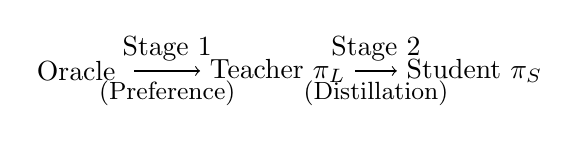
\begin{tikzpicture}[node distance=2.5cm, auto]
\node (oracle) {Oracle $\fstar$};
\node (teacher) [right of=oracle] {Teacher $\pi_L$};
\node (student) [right of=teacher] {Student $\pi_S$};
\draw[->] (oracle) -- node[above] {Stage 1} node[below] {\small (Preference)} (teacher);
\draw[->] (teacher) -- node[above] {Stage 2} node[below] {\small (Distillation)} (student);
\end{tikzpicture}
\end{center}

\paragraph{Stage 1: Preference Learning.}
Train a large policy $\pi_L$ via DPO/GRPO on oracle-preserving summaries $Z^{(R)}(X)$.

\paragraph{Stage 2: Distillation.}
Train a smaller policy $\pi_S$ to match $\pi_L$, using the same summaries.

\subsection{Proof Strategy Overview}

The pipeline composition analysis uses a simple but powerful technique: \textbf{chaining triangle inequalities across stages}.

\paragraph{Core Insight.}
Each stage introduces a gap, but these gaps compose \emph{additively} rather than multiplicatively. The key observation is that the same metric (expected loss) is used throughout, so we can chain:
\[
\text{Student on full} \approx \text{Student on summary} \approx \text{Teacher on summary} \approx \text{Teacher on full}.
\]

\paragraph{Role of Oracle-Measurability.}
The assumption that both student and teacher are oracle-measurable ensures that the summarization gap $\epsilon_1$ applies symmetrically to both models. Without this, the student might introduce additional approximation error from the summarization step.

\paragraph{Generalization to $K$ Stages.}
The composition is fundamentally additive because the triangle inequality is additive. Each new stage adds at most two terms: one for summarization (if summaries are used) and one for the stage-specific transformation (distillation, fine-tuning, etc.).

\subsection{Abstract Gap Composition}

\begin{theorem}[Training Path Gap Bound]\label{thm:path-gap}
Let $\mathcal{L}(\pi; \mu)$ denote the expected loss of policy $\pi$ on distribution $\mu$. Suppose:
\begin{align}
\epsilon_1 &:= |\mathcal{L}(\pi_L; \mu_X) - \mathcal{L}(\pi_L; \mu_Z)| & \text{(Stage 1 gap)} \\
\epsilon_2 &:= |\mathcal{L}(\pi_S; \mu_Z) - \mathcal{L}(\pi_L; \mu_Z)| & \text{(Stage 2 gap)}
\end{align}
If the student also satisfies $|\mathcal{L}(\pi_S; \mu_X) - \mathcal{L}(\pi_S; \mu_Z)| \le \epsilon_1$, then:
\[
|\mathcal{L}(\pi_S; \mu_X) - \mathcal{L}(\pi_L; \mu_X)| \le 2\epsilon_1 + \epsilon_2.
\]
\end{theorem}

\begin{proof}
By the triangle inequality:
\begin{align*}
|\mathcal{L}(\pi_S; \mu_X) - \mathcal{L}(\pi_L; \mu_X)|
&\le |\mathcal{L}(\pi_S; \mu_X) - \mathcal{L}(\pi_S; \mu_Z)| \\
&\quad + |\mathcal{L}(\pi_S; \mu_Z) - \mathcal{L}(\pi_L; \mu_Z)| \\
&\quad + |\mathcal{L}(\pi_L; \mu_Z) - \mathcal{L}(\pi_L; \mu_X)| \\
&\le \epsilon_1 + \epsilon_2 + \epsilon_1 = 2\epsilon_1 + \epsilon_2.
\end{align*}
\end{proof}

\subsection{Exact Preservation Case}

When local laws hold exactly ($\Delta_R = 0$), Stage 1 has zero gap.

\begin{corollary}[Exact Preservation Distillation]
If $\metric(\fstar(Z^{(R)}(X)), \fstar(X)) = 0$ almost surely and the student satisfies the same oracle-measurability conditions as the teacher, then:
\[
|\mathcal{L}(\pi_S; \mu_X) - \mathcal{L}(\pi_L; \mu_X)| = \epsilon_2,
\]
i.e., the end-to-end gap equals the pure distillation gap.
\end{corollary}

\subsection{Quantitative Bounds}

Under approximate preservation with $\Delta_R > 0$:

\begin{theorem}[Quantitative Pipeline Bound]
Let $L$ be the Lipschitz constant for the preference learning loss (from Appendix~\ref{sec:grpo}). Then:
\[
\epsilon_1 \le L \cdot \Delta_R,
\]
and the end-to-end gap is:
\[
|\mathcal{L}(\pi_S; \mu_X) - \mathcal{L}(\pi_L; \mu_X)| \le 2 L \Delta_R + \epsilon_2.
\]
\end{theorem}

\subsection{Multi-Stage Extensions}

The composition extends to $K$-stage pipelines:

\begin{theorem}[$K$-Stage Composition]
For a pipeline $\pi_0 \to \pi_1 \to \cdots \to \pi_K$ with per-stage gaps $\epsilon_1, \ldots, \epsilon_K$:
\[
|\mathcal{L}(\pi_K; \mu_X) - \mathcal{L}(\pi_0; \mu_X)| \le 2(K-1)\epsilon_1 + \sum_{k=2}^K \epsilon_k,
\]
where $\epsilon_1$ is the summarization gap (applied at each stage where summaries are used) and $\epsilon_k$ for $k \ge 2$ are distillation/fine-tuning gaps.
\end{theorem}

\begin{proof}
We prove by induction on $K$. For $K=2$ the claim is Theorem~\ref{thm:path-gap}. Assume the bound holds for $K-1$ stages. Consider the $K$-stage pipeline as a $(K-1)$-stage chain ending at $\pi_{K-1}$ followed by the final stage $\pi_{K-1}\to\pi_K$. By the inductive hypothesis,
\[
|\mathcal{L}(\pi_{K-1}; \mu_X) - \mathcal{L}(\pi_0; \mu_X)|
\le 2(K-2)\epsilon_1 + \sum_{k=2}^{K-1} \epsilon_k.
\]
Applying the two-stage bound to the final stage yields
\[
|\mathcal{L}(\pi_K; \mu_X) - \mathcal{L}(\pi_{K-1}; \mu_X)|
\le 2\epsilon_1 + \epsilon_K.
\]
By the triangle inequality, the two displays combine to give
$|\mathcal{L}(\pi_K; \mu_X) - \mathcal{L}(\pi_0; \mu_X)|
\le 2(K-1)\epsilon_1 + \sum_{k=2}^K \epsilon_k$.
\end{proof}

\subsection{Distillation Gap Analysis}

The distillation gap $\epsilon_2$ depends on:
\begin{itemize}[nosep]
    \item \textbf{Capacity gap}: How much expressive power the student loses
    \item \textbf{Optimization gap}: How well distillation recovers the teacher's behavior
    \item \textbf{Distribution shift}: Differences between training and test distributions
\end{itemize}

\begin{definition}[Distillation Loss]
The distillation objective minimizes:
\[
\mathcal{L}_{\text{distill}}(\pi_S) = \E_{x \sim \mu_Z} \left[ D_{\text{KL}}(\pi_L(\cdot \mid x) \| \pi_S(\cdot \mid x)) \right].
\]
\end{definition}

\begin{theorem}[Distillation to DPO Transfer]
If $\mathcal{L}_{\text{distill}}(\pi_S) \le \epsilon_{\text{distill}}$, then under mild regularity conditions:
\[
|\mathcal{L}_{\text{DPO}}(\pi_S; \mu_Z) - \mathcal{L}_{\text{DPO}}(\pi_L; \mu_Z)| \le C \cdot \sqrt{\epsilon_{\text{distill}}},
\]
where $C$ depends on the DPO temperature $\beta$ and action space size.
\end{theorem}

\begin{proof}
By Pinsker's inequality,
\[
D_{\text{TV}}(\pi_L(\cdot\mid x),\pi_S(\cdot\mid x))
\le \sqrt{\tfrac12 D_{\text{KL}}(\pi_L(\cdot\mid x)\,\|\,\pi_S(\cdot\mid x))}.
\]
Taking expectations and applying Jensen gives
$\E_x[D_{\text{TV}}(\pi_L,\pi_S)]\le \sqrt{\epsilon_{\text{distill}}/2}$.
Assume a uniform lower bound on action probabilities under the reference and student policies so that log-ratios are Lipschitz in total variation:
$
|\log \pi_S(a\mid x)-\log \pi_L(a\mid x)|\le C_0\,D_{\text{TV}}(\pi_L,\pi_S).
$
Because $-\log\sigma$ is 1-Lipschitz, the per-sample DPO loss difference is bounded by a constant times the logit difference, hence by $C_1 D_{\text{TV}}(\pi_L,\pi_S)$. Averaging over $x$ yields
\[
|\mathcal{L}_{\text{DPO}}(\pi_S;\mu_Z)-\mathcal{L}_{\text{DPO}}(\pi_L;\mu_Z)|
\le C_1\,\E_x[D_{\text{TV}}(\pi_L,\pi_S)]
\le C\,\sqrt{\epsilon_{\text{distill}}},
\]
for $C=C_1/\sqrt{2}$.
\end{proof}

\subsection{Practical Recommendations}

\paragraph{Stage 1: Maximize Teacher Quality.}
Invest in:
\begin{itemize}[nosep]
    \item Driving $\Delta_R$ low via audit-driven prompt optimization
    \item Using the largest feasible teacher model
    \item Collecting high-quality preference data on summaries
\end{itemize}

\paragraph{Stage 2: Minimize Distillation Gap.}
\begin{itemize}[nosep]
    \item Use sufficient student capacity for the task
    \item Train on diverse summaries covering the input distribution
    \item Validate distillation quality on held-out summaries
\end{itemize}

\paragraph{End-to-End Validation.}
After deployment, sample full documents and verify:
\[
\hat{\epsilon}_{\text{e2e}} = \frac{1}{n} \sum_{i=1}^n |\mathcal{L}(\pi_S; x_i) - \mathcal{L}(\pi_L; x_i)|
\]
against the theoretical bound $2L\Delta_R + \epsilon_2$.
